\documentclass[journal=jpcafh]{achemso}
\usepackage{achemso}
\setkeys{acs}{maxauthors = 10 }
\usepackage{amsmath}
\usepackage{rotating}
\usepackage{multirow}
\usepackage{tabularx}
\usepackage{esvect}
\usepackage{bm}
\usepackage[export]{adjustbox}
\usepackage{longtable}
\usepackage{lscape}
\usepackage[T1]{fontenc}
\usepackage[colorinlistoftodos]{todonotes}
\usepackage{subcaption}


\SectionNumbersOn
\newcommand{\rotunits}{deg dm$^{-1}$ (g/mL)$^{-1}$}


\author{J. Coleman Howard}
\affiliation{Department of Chemistry, Virginia Tech, Blacksburg, VA 24061, USA}
\author{T. Daniel Crawford}
\affiliation{Department of Chemistry, Virginia Tech, Blacksburg, VA 24061, USA}
\email{crawdad@vt.edu}

{\title{Calculating Optical Rotatory Dispersion Spectra in Solution Using a Smooth
Dielectric Model}
\begin{document}
\begin{abstract}
The calculation of specific rotation of molecules in solution is probed at
the coupled cluster (CC) level utilizing a continuum dielectric model
based on a definition of the dielectric permittivity as a smooth function
of electron density. Solvation effects are captured through
polarization of Hartree-Fock (HF) molecular orbitals before subsequent
calculations with the coupled cluster singles and doubles (CCSD) method.
For the challenging (\emph{S})-methyloxirane molecule, CCSD specific rotations
yield an incorrect sign for the rotation in water, and the
continuum model is unable to predict the wide variations in the optical
rotatory dispersion (ORD) curves seen for nonpolar solvents of similar
dielectric constant. In two molecules, (\emph{1S,4S})-norbornenone and
(\emph{S})-2-chloropropionitrile, specific rotations computed with CCSD
in conjunction with implicit solvent fail to provide solvent shifts 
of the correct order of magnitude, indicating that the solvent response
is a major contribution to the overall solvation effect.
\end{abstract}

\newpage
\section{Introduction}
Successfully modeling chiroptical properties such as optical rotation
ostensibly requires the same
theoretical considerations involved in modeling any molecular property,
e.g., choices in atomic orbital (AO) basis sets and approaches to electron
correlation effects. Optical rotation calculations, however, demonstrate
a particular sensitivity to these theoretical details and others,
including the treatment of
the environment surrounding a chiral molecule, and represent an ongoing challenge
to theoretical quantum chemistry.\cite{Crawford:06,Srebro:17,Crawford:18}
Highly correlated quantum mechanical
(QM) methods\cite{Shavitt:09,Crawford:00,Helgaker:12} offer the most reliable means of calculation, however
even an accurate correlated
method such as the coupled cluster singles and doubles (CCSD) method
can produce specific rotation values significantly at odds with experimental
results.
One difficulty in comparing accurate QM wavefunction methods with
experiment is that especially large, flexible AO basis sets
are needed to obtain converged optical rotation values near the complete basis
set (CBS) limit,\cite{Mach:11,Baranowska:13,Haghdani:16} and, in contrast to many
molecular properties,\cite{Papajak:11} diffuse basis functions are of
critical importance in optical rotation calculations.\cite{Baranowska:10,
Mach:11,Wiberg:13}
Even with a sufficient treatment of dynamical electron correlation and a basis set
approaching the CBS limit, a single optical rotation calculation on
a molecular system in its minimum-energy geometry may be an inappropriate 
comparison to an experimental value. For example, it is known that
vibrational corrections to specific rotation can be significant,\cite{Ruud:01,
Ruud:05,Mort:05,Kongsted:08,Pedersen:09,Pedersen:09b} even to the
extent that the molecular vibrations induce sign changes at points in the optical
rotatory dispersion (ORD) curve.\cite{Ruud:05}
For conformationally flexible molecules, a great number of conformations
may need to be considered
depending on the experimental conditions.\cite{Wiberg:03,Wiberg:05,
Lambert:12,Pearce:17}

In addition to these factors, the role of solvent is understood to be
of primary importance in ORD spectra.\cite{Kumata:70,Berova:00}
The specific rotation of a molecule measured in the gas phase can differ
drastically from the rotation in solution or the condensed phase,
even changing sign depending on the solvent.\cite{Kumata:70,Wilson:05}
In contrast to many other properties where nonpolar solvent environments
are expected to more closely mimic conditions in the gas phase
relative to polar solvents, the opposite can be true for measured specific
rotations.\cite{Wilson:05} An additional complication in modeling
rotation in solution is that the structure of the surrounding solvent molecules
itself may also contribute to specific rotation, as the ``chiral
imprint'' can be responsible for a significant portion of the solvent
shift.\cite{Beratan:06,Beratan:07} A more complete understanding of the
nature of these solvent effects 
is essential to increasing the reliability of theoretical
optical rotation predictions across all phases.

Solvent effects have been incorporated into optical rotation calculations
often with an implicit solvation approach, such as the
venerable polarizable continuum model (PCM).\cite{Miertus:81,Tomasi:05}
Often used in conjunction with density functional theory (DFT) methods,
DFT/PCM treatments have yielded mixed results in specific rotation
calculations in comparison to experimental values.\cite{Mennucci:02,
Kongsted:08,Lahiri:13}
An explicit treatment of solvent molecules has the advantage of capturing
specific solute-solvent interactions inaccessible to a continuum model,
(e.g., hydrogen bonding). The inclusion of explicit solvent effects
has contributed valuable insight into the role of solvent molecules
in methyloxirane's optical rotation, probing the contributions of
the dissymmetric solvent structure,\cite{Beratan:06,Beratan:07}
as well as achieving quantitative agreement with experimental measurements
in water when combined with an implicit treatment of the bulk solvent
and vibrational corrections.\cite{Lipparini:13} Unfortunately, 
explicit solvation treatments require extensive sampling of configurations, 
and typically thousands of molecular dynamics snapshots are needed for converged
results.\cite{Beratan:06,Beratan:07,Lipparini:13} The associated computational
cost of of such an approach necessarily limits the applicability of most
wavefunction-based electronic structure methods, and one often relies on
DFT methods, where gas-phase specific rotation results, for methyloxirane
in particular, depend on significant error cancellation to obtain correct
signs.\cite{Kongsted:06} In this work, we investigate the combination of
coupled-cluster linear response theory and an implicit solvation model
based on a smooth definition of the dielectric permittivity to obtain
specific rotation values in solution.

The implicit solvent model utilized herein is based on a definition
of the dielectric permittivity as a function of electron density. 
Introduced by Fattebert and Gygi\cite{Fattebert:02,Fattebert:03},
this model was developed for use in the context of plane-wave based DFT
calculations
\cite{Scherlis:06,Andreussi:12,Dziedzic:11,Dziedzic:13,Fox:14}
and has been particularly successful in computing accurate solvation
energies relative to contemporary solvent models.\cite{Dziedzic:11,
Dziedzic:13}
The definition of the dielectric permittivity takes the form of Equation
\ref{eqn:eps}.

\begin{align}
\epsilon[\rho({\mathbf{r}})] = 1 + \frac{\epsilon_\infty-1}{2}\left[1+\frac{1-\left(
\rho({\mathbf{r}})/\rho_0\right)^{2\beta}}{1+(\rho({\mathbf{r}})/\rho_0)^
{2\beta}}\right]
\label{eqn:eps}
\end{align}
In this model, the dielectric permittivity $\epsilon$ is determined by the
electron density
($\rho$) and depends on the two parameters $\rho_0$ and $\beta$, which
control the transition of $\epsilon$ from the vacuum value of one to the
dielectric constant of the bulk solvent $\epsilon_\infty$. The appropriate electrostatic problem
in this case corresponds to solving the generalized Poisson equation (GPE)
(Equation \ref{eqn:GPE}) for the electrostatic potential ($V^\mathrm{GPE}$).

\begin{align}
\nabla \cdot  \left[ \epsilon({\mathbf{r}})\nabla V^\mathrm{GPE}({\mathbf{r}})\right] = 
-4\pi \rho_\mathrm{tot}({\mathbf{r}})
\label{eqn:GPE}
\end{align}
Unlike the standard Poisson equation corresponding to electrostatics in vacuum
or a homogeneous permittivity, which can be solved analytically,
the GPE in Equation \ref{eqn:GPE} must in general be solved by numerical
techniques. Its solution here is achieved by interfacing with 
DL\_MG,\cite{Womack:18} an open-source multigrid solver library. As previously
described,\cite{Howard:17} real-space grid representations of the permittivity
and total density $\rho_\mathrm{tot}$ are used to obtain $V^\mathrm{GPE}$,
which is numerically integrated into the AO basis and iterated to self-consistency
along with the HF molecular orbitals.
We have previously\cite{Howard:17} incorporated this continuum
solvent model in a Hartree-Fock framework to extend its use to
correlated wavefunction methods.
A study of small molecules with well-known electronic excitation
solvent shifts demonstrated good performance for this solvation model
in conjunction with the EOM-CCSD method, typically reproducing experimentally
determined n$\rightarrow \pi^*$ blue shifts to within 0.1 eV.\cite{Howard:17}
This continuum dielectric model requires only two parameters and,
capturing the effects of solvation through the molecular orbitals
and Fock matrix elements (analogous to a PTE approximation in PCM)
\cite{Lipparini:16,Cammi:13},
can be readily extended to any post-HF
correlated method.  This approach can be contrasted with a more complete
treatment of continuum solvation at the correlated level, which
would include the solvent's response to electron correlation and/or the
electric and magnetic field perturbations, as well as a proper
consideration of non-equilibrium solvation effects, as has been demonstrated
by Caricato.\cite{Caricato:13} Despite the present model's relative simplicity,
excitation energies computed via EOM-CCSD calculations in solution have
compared favorably with those resulting from more sophisticated approaches.
\cite{Howard:17} In this work, we apply this smooth dielectric model
(hereafter, referred to as the FGS model)
to the computation of specific rotations in solution at the CCSD level.


\section{Computational Methods}
Specific rotation values were computed with the CCSD method for three
molecules, (\emph{S})-methyloxirane, (\emph{1S,4S})-norbornenone, and
(\emph{S})-2-chloropropionitrile using the aug-cc-pVDZ basis set.
\cite{Kendall:92}
Each of these calculations utilize
the velocity-gauge representation of the dipole operator, ensuring
origin-independent results, and all reported specific rotation values represent
modified velocity-gauge results.\cite{Pedersen:04b}
Each of these geometries was optimized with the B3LYP DFT functional
using the 6-311G(d,p) basis set.\cite{Krishnan:80} The core orbitals
(i.e., 1$s$ for C,N, and O; $1s2s2p$ for Cl) were kept frozen
in the CCSD energy and response calculations.
In defining the dielectric permittivity according to Equation \ref{eqn:eps},
the solvent cavity was fixed based on a converged electronic SCF density
computed in vacuum, as in Reference \citenum{Howard:17}. For selecting
the dimensions of the real-space grid used in solving the GPE for the
electrostatics in solution, the number of points and grid spacing were
selected such that specific rotations computed in vacuum with electrostatic
computed from the GPE reproduced those from a conventional CCSD specific
rotation calculation. For the three molecules studied here, the maximum
deviation between those rotation values is less than 4 \rotunits, and
corresponds to the specific rotation of (1\emph{S},4\emph{S})-norbornenone
at 355 nm, which has a magnitude greater than 3000 \rotunits. The values of the electrostatic potential on the boundary points of the grid are approximated by computing the potential associated with a homogeneous medium of $\epsilon$ corresponding to the solvent's dielectric constant, as in previous works.\cite{Dziedzic:11,Howard:17} The grid
details, as well as parameters used in the DL\_MG multigrid calculations,
are provided in the Supporting Information. For the PCM calculations performed
here, geometry optimizations were performed with Gaussian09 software
\cite{g09}. All other computations were performed with the Psi4 software
package,\cite{psi4} utilizing an interface to PCMSolver\cite{pcmsolver}
for specific rotation calculations with PCM solvents. Those calculations
utilized PCM cavities constructed with Bondi radii scaled by a factor of 1.2.

\newpage
\section{Results and Discussion}
\begin{table}[h]
\caption{Specific rotations (\rotunits) of (\emph{S})-methyloxirane computed
in vacuum and shifts computed in solvents at the CCSD/aug-cc-pVDZ level
}
\begin{tabular*}{\linewidth}{@{\extracolsep{\fill}}cccccccc@{}}
  \hline \hline
&Vacuum &C$_6$H$_{12}$ &CCl$_4$&C$_6$H$_6$ &CH$_3$CH$_2$OH &CH$_3$CN  &H$_2$O \\
$\lambda$ (nm)
       &$[\alpha]_\omega$ &$\Delta [\alpha]_\omega$  &$\Delta [\alpha]_\omega$ 
&$\Delta [\alpha]_\omega$ &$\Delta [\alpha]_\omega$
&$\Delta [\alpha]_\omega$ &$\Delta [\alpha]_\omega$ \\
\hline
253 & 104.2 & -1.6  & -0.8 & -0.6 &+41.2 &+47.9 &+63.1 \\
302 & -42.8 &+11.5  &+13.3 &+13.6 &+52.0 &+56.5 &+66.2 \\
365 & -59.3 &+10.1  &+11.5 &+11.8 &+38.6 &+41.4 &+47.5 \\
436 & -50.1 & +7.5  & +8.5 & +8.7 &+27.2 &+29.0 &+33.0 \\
546 & -35.2 & +4.9  & +5.5 & +5.6 &+17.1 &+18.2 &+20.7 \\
578 & -31.9 & +4.3  & +4.9 & +5.0 &+15.2 &+16.2 &+18.4 \\
589 & -30.9 & +4.2  & +4.7 & +4.8 &+14.7 &+15.6 &+17.6 \\
\hline \hline
\end{tabular*}
\label{table:smo}
\end{table}

The case of methyloxirane perhaps best exemplifies the large role solvent
effects can play in optical rotation. Since the work of Kumata
\emph{et al.},\cite{Kumata:70} it has been recognized that the solvent
environment has a significant effect on the ORD curve of methyloxirane. 
These and subsequent experiments have revealed qualitatively different
shapes for the ORD curves in benzene compared to those in polar
solvents water and acetonitrile.\cite{Kumata:70,Wilson:05}
At a wavelength of 302 nm, the specific rotation of
(\emph{S})-methyloxirane in benzene is nearly -100 \rotunits, while, in water,
the measured rotation is around +60 \rotunits.\cite{Wilson:05} Specific rotations
measured at several wavelengths  on the ORD curve
for a variety of other solvents produce a range of
rotation values intermediate between these two solvents,
\cite{Kumata:70,Wilson:05} and available gas-phase measurements
lie closer to those in more polar solvents in this case.\cite{Wilson:05}

A variety of computational efforts have addressed the problem of
methyloxirane's specific rotation in solvent. Mennucci \emph{et al.}
\cite{Mennucci:02}
examined solvent effects on the rotation of several molecules,
including methyloxirane, presenting the first demonstration of
electronic structure calculations of optical rotation to employ 
PCM to model the solvent environment. Despite the success of PCM
in modeling a variety of molecular properties,\cite{Tomasi:05}
B3LYP\cite{Becke:93,Lee:88,Stephens:94} PCM calculations were incapable of reproducing the experimental
ordering of specific rotations in different solvents. B3LYP PCM
calculations have also been combined with zero-point vibrational
corrections in methyloxirane,\cite{Kongsted:08} resulting in
improvements in the computed solvent shifts in cyclohexane relative
to experiment. For more polar solvents, however, that methodology was
unable to model the correct relative shifts observed experimentally.
Beyond density functional theory, optical rotation of methyloxirane
in solution has also been investigated at the coupled-cluster level,
including correlation up to an approximation of triple excitations
in the CC3 method.\cite{Kongsted:05} In conjunction with a spherical
cavity dielectric model in CC/DC computations,\cite{Kongsted:05} 
those highly correlated methods also failed to predict the observed trends
across a variety of solvents.

Table \ref{table:smo} summarizes the results of CCSD/aug-cc-pVDZ specific
rotation values of (\emph{S})-methyloxirane computed in vacuum, as well
as in a variety of solvents treated as a continuum dielectric. The wavelengths
in the first column cover a range of values for which experimental measurements
are available. The CCSD/aug-cc-pVDZ specific rotation values for the isolated
molecule are given by the second column of Table \ref{table:smo}. At 253
nm, the vacuum rotation value is +104.2 \rotunits, becoming more negative
at -59.3 \rotunits \ as the wavelength increases to 365 nm. At longer wavelengths,
the vacuum rotation remains negative, reaching -30.9 \rotunits \ at 589 nm.
The remaining columns of Table \ref{table:smo} give the  solvent shifts computed
with the FGS model in combination with CCSD response calculations, relative
to the CCSD vacuum rotations. For the nonpolar solvents cyclohexane, carbon
tetrachloride, and benzene (third through fifth columns), the predicted
shifts are on the order of several \rotunits. The large positive rotation
at 253 nm is shifted only slightly smaller in each of these solvents, and none of
the shifts exceed 2 \rotunits. The negative specific rotations near 300 nm
all undergo larger shifts towards more positive values in the nonpolar environments, the magnitude of these shifts ranging from $+4$ to $+14$ \rotunits, with the
largest shifts due to the rotations calculated at 302 nm and 365 nm.
For the three polar solvents considered here (ethanol, acetonitrile, and water),
the specific rotation shifts relative to vacuum CCSD values are much larger.
At all wavelengths, the shifts are positive (last three columns of \ref{table:smo}). The predicted specific rotation shifts in water at
253 nm and 302 nm
exceed $+60$ \rotunits, a shift which is larger than the magnitude of any
of the negative vacuum specific rotation values above 300 nm.


\begin{figure}
\begin{subfigure}{.45\textwidth}
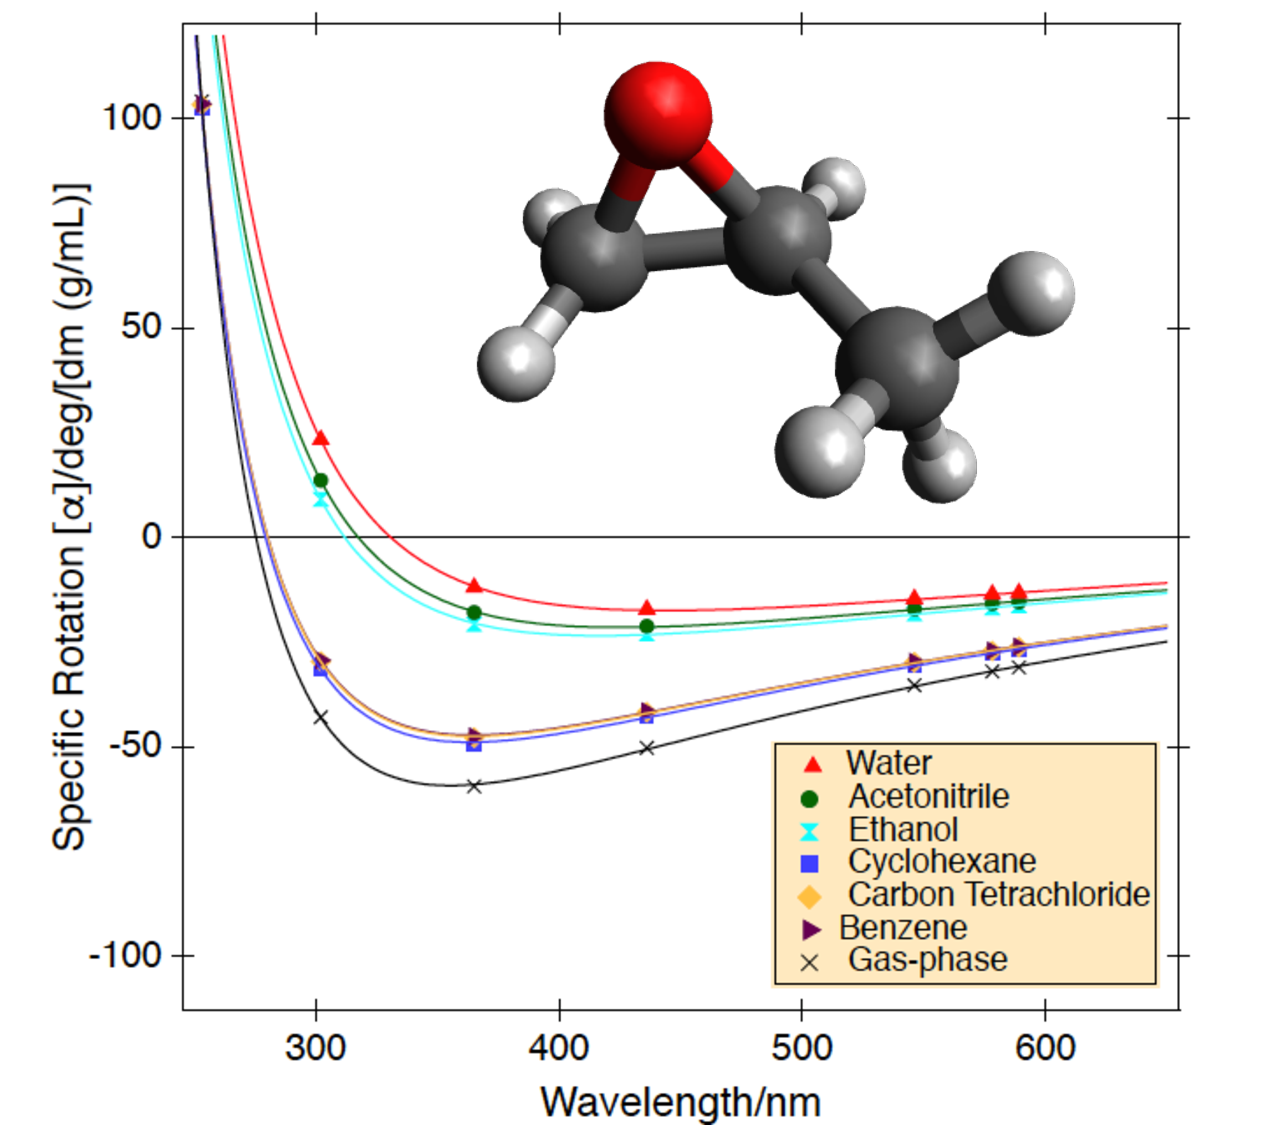
\includegraphics[width=2.5in]{figs/fig1a.pdf}
\caption*{\hspace{-1.25em}(a)}
\end{subfigure}
\hfill
\begin{subfigure}{.45\textwidth}
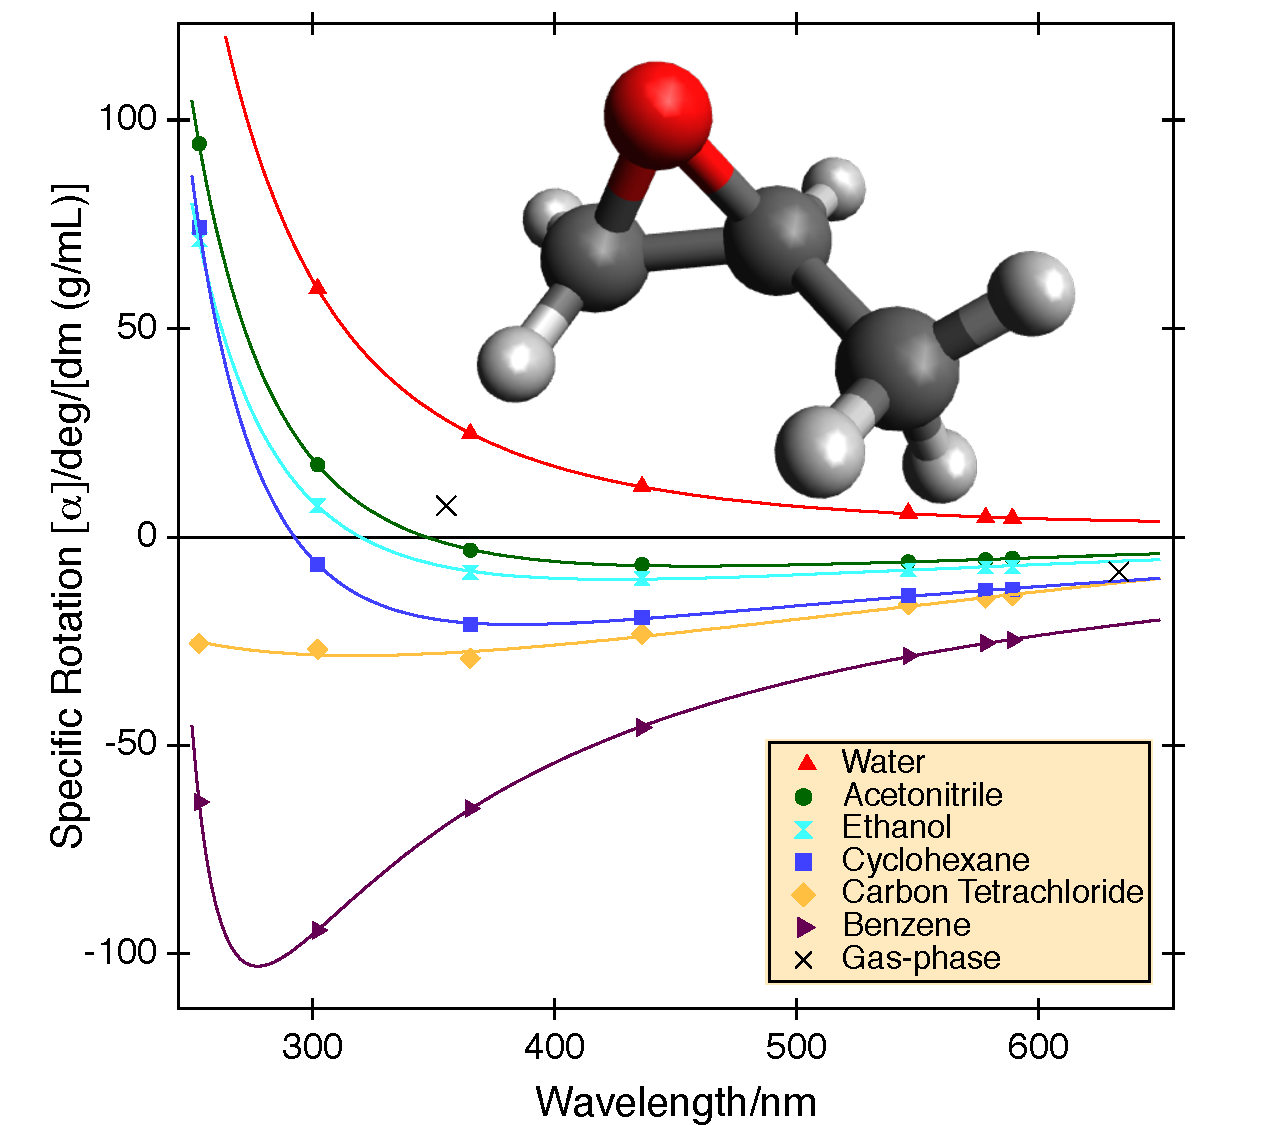
\includegraphics[width=2.5in]{figs/fig1b.pdf}
\caption*{\hspace{-1.25em}(b)}
\end{subfigure}
\caption{Optical rotatory dispersion curves of (\emph{S})-methyloxirane
(a) computed at the CCSD/aug-cc-pVDZ level with various solvents
and (b) from experimentally determined values\cite{Wilson:05}
}
\label{fig:smo}
\end{figure}

Figure \ref{fig:smo} displays the ORD curves for (\emph{S})-methyloxirane in
various solvents, including those computed at the CCSD/aug-cc-pVDZ level
in implicit solvent with the FGS model in Figure 1(a) and from experimental
determinations in Figure 1(b).
\cite{Wilson:05} The experimental rotation values display a wide
range
across all solvents, with the most polar solvents (water and acetonitrile)
showing positive rotations above 50 \rotunits\ at wavelengths
below 300 nm. In benzene,
the rotation of (\emph{S})-methyloxirane shifts to nearly -100 \rotunits\
in the same wavelength range experimentally. Comparing the CCSD/aug-cc-pVDZ
specific rotations computed in solution using the smooth FGS model (Figure
1(a)),
the relative ordering of the polar solvents water, acetonitrile, and ethanol
is correct, and the computed ORD curves display a qualitative agreement
with experiment for most of the polar solvents.
However, there are clearly major discrepancies in the calculated
and experimental curves. For example, the experimental ORD curve of (\emph{S})-methyloxirane
in water is positive at all wavelengths, while the values computed here
predict negative rotations above 302 nm. For the remaining solvents,
the sign of the rotation is correctly predicted, although the actual
values can deviate significantly from experiment, such as in benzene,
where the computed rotation value is too large at 302 nm by more than 60
\rotunits. In addition, because of the similar dielectric constants
of the nonpolar solvents here, the implicit solvent calculations are unable
to predict the variations seen experimentally among the ORD curves in nonpolar solvents.

In evaluating the quality of the CCSD calculations with the
FGS model, the shifts relative to vacuum are perhaps the most important,
since the absolute specific rotations in solution may benefit from
error cancellation in regards to basis set incompleteness, a lack of
vibrational corrections, etc. The experimental vacuum values\cite{Wilson:05}
are 7.49 \rotunits at 355 nm and -8.39 \rotunits at 633 nm (marked with
black X's in Figure 1). The CCSD/aug-cc-pVDZ vacuum values,
on the other hand, are represented by the most negative computed ORD curve.
At these two points, then, almost all of the computed shifts in Table 1
are in the wrong direction, with only the calculations in water solvent
correctly predicting positive shifts in the rotation. The unsatisfactory
performance of the CCSD shifts computed with the FGS model are in line
with previous efforts to apply continuum solvation to the problem of
methyloxirane's rotation in solution. The B3LYP PCM shifts
computed at 589 nm by Mennucci \emph{et al.}\cite{Mennucci:02}
agree with the CCSD FGS computed shifts for the nonpolar solvents
to within 2 \rotunits, while the acetonitrile shift computed in this work
are a bit more positive (by $+8$ \rotunits). Solvents shifts at 355
nm, also with B3LYP and PCM, were reported by Kongsted \emph{et al.}\cite{Kongsted:08}
and a similar shift was seen to that computed here at 365 nm in cyclohexane,
while the CCSD FGS results again predict larger shifts
in polar solvents compared to a DFT with PCM approach. 
Importantly, Kongsted \emph{et al.}
noted the importance of vibrational contributions to the shifts themselves,
as the effect was large enough in the case of cyclohexane to change the sign
of the computed shift at long wavelengths.\cite{Kongsted:08}
In contrast to the present CCSD results with the FGS model,
a previous attempt to model the solvents with a continuum model at the
CCSD level\cite{Kongsted:06} utilizing the CC/DC model predicts small, negative
shifts in the specific rotations of (\emph{S})-methyloxirane at 355 nm
for the nonpolar solvents examined here, in better accord with the experimental
picture and likely an improvement due to the CC/DC approach incorporating
the response of the solvent environment into the CC response equations.
\cite{Christiansen:99}

\begin{figure}
\begin{subfigure}{.4\textwidth}
\hspace{0.5in}
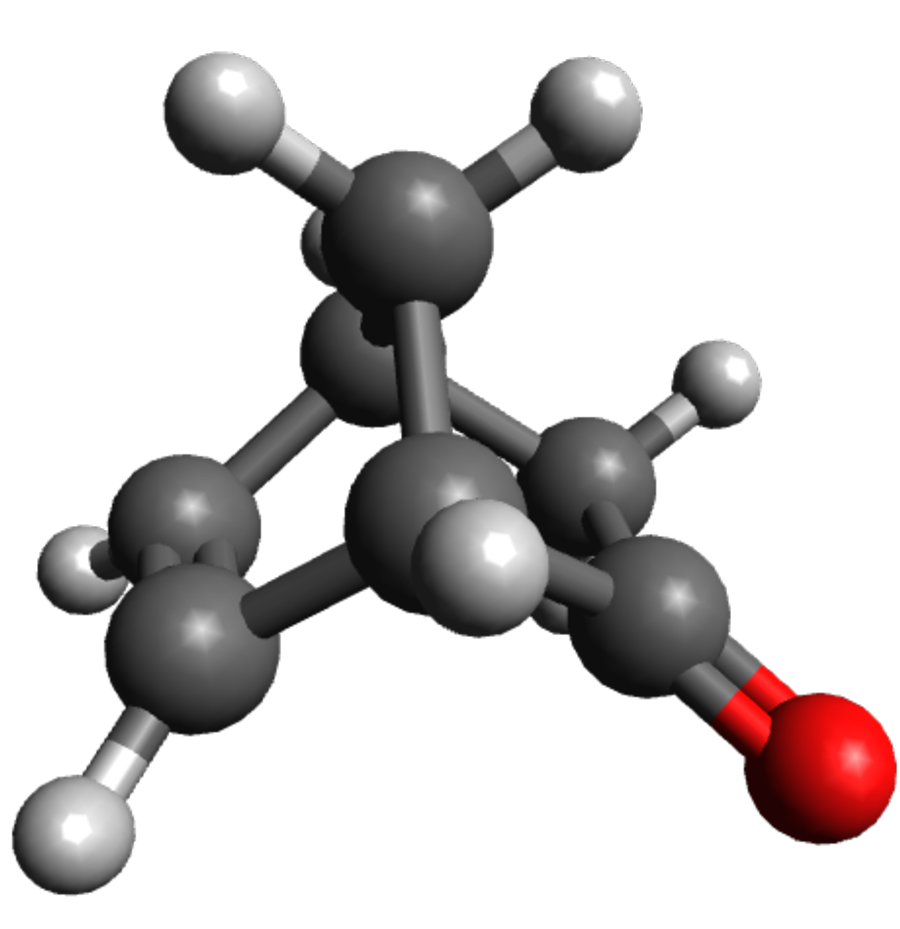
\includegraphics[width=1.75in]{figs/fig2a.pdf}
\caption*{\hspace{1.5em}(a)}
\end{subfigure}
\hfill
\begin{subfigure}{.4\textwidth}
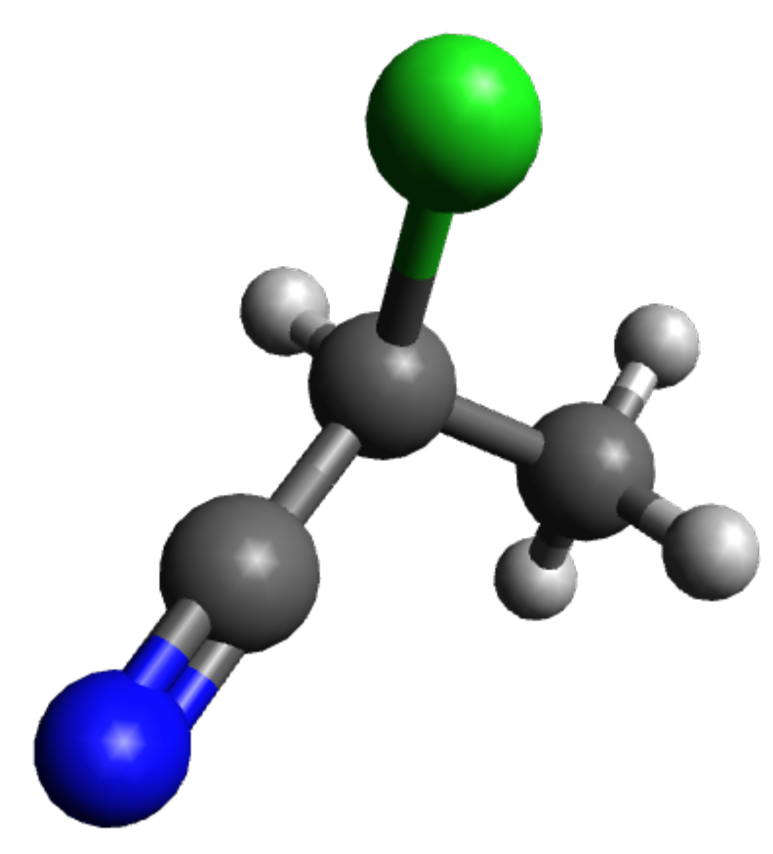
\includegraphics[width=1.75in]{figs/fig2b.pdf}
%\hfill
\caption*{\hspace{-5em}(b)}
\end{subfigure}
\caption{Two molecules studies in this work: (a) (\emph{1S},\emph{4S})-norbornenone
and (b) (\emph{S})-2-chloropropionitrile
}
\label{fig:other_molecules}
\end{figure}



Norbornenone is a molecule which has attracted theoretical interest due to
its very large-magnitude
specific rotation values relative to structurally similar chiral molecules.
\cite{Stephens:01,Ruud:03,Mach:11,Moore:12,Lahiri:13,Caricato:14}
The especially large rotation value has been analyzed in terms of the
excited state contributions\cite{Caricato:14}, as well as the contributions
from specific localized orbitals, and the lowest excited
state appears to be largely responsible for the sizable rotation,\cite{Caricato:14}
with a favorable alignment of the carbonyl and alkenyl groups playing a significant
role.\cite{Moore:12,Caricato:14} Modeling the
specific rotation of the isolated norbornenone molecule has been a challenge
and shows a strong dependence on theoretical method. DFT
\cite{Stephens:01,Ruud:03,Moore:12,Lahiri:13,Caricato:14}
and CC calculations\cite{Ruud:03,Mach:11,Lahiri:13} provide vastly
different rotation values, and at 355 nm, the experimental value of -6310
\rotunits \ is between B3LYP and CCSD results, which both deviate from
experiment by more than 2000 \rotunits.\cite{Lahiri:13}

\begin{table}[h]
\caption{Specific rotations (\rotunits) of (\emph{1S,4S})-norbornenone computed
in vacuum and shifts computed in solvents at the CCSD/aug-cc-pVDZ level
}
\begin{tabular*}{\linewidth}{@{\extracolsep{\fill}}cccccccc@{}}
  \hline \hline
& &\multicolumn{2}{c}{CCSD} &\multicolumn{2}{c}{PCM-B3LYP$^a$}
&\multicolumn{2}{c}{Experiment$^a$} \\
\cline{3-4} \cline{5-6} \cline{7-8}
&Vacuum &C$_6$H$_{12}$ &CH$_3$CN &C$_6$H$_{12}$ &CH$_3$CN 
&C$_6$H$_{12}$ &CH$_3$CN 
\\
$\lambda$ (nm) &$[\alpha]_\omega$
&$\Delta [\alpha]_\omega$ &$\Delta [\alpha]_\omega$ 
&$\Delta [\alpha]_\omega$ &$\Delta [\alpha]_\omega$ 
&$\Delta [\alpha]_\omega$ &$\Delta [\alpha]_\omega$ \\
\hline
355 &-3732.2 &+44.6 &+131.8 &-1066 &-855	&-2849  &-2297 \\
436 &-1429.4 &-4.9  &-15.0  &-- &--		&--  &-- \\
589 & -551.7 &-5.5  &-16.8  &-152 &-118		&-226  &-195 \\
633 & -454.5 &-4.8  &-14.9	&-125 &-96 	&-182  &-159 \\
\hline \hline
\multicolumn{8}{l}{$^a$ Reference \citenum{Lahiri:13}}
\end{tabular*}
\label{table:norb}
\end{table}

Norbornenone also undergoes a significant solvation effect, which is
under investigation here. Table \ref{table:norb} provides the calculated
CCSD/aug-cc-pVDZ vacuum rotations and shifts computed with the FGS
continuum treatment of solvent effects. For additional comparison, the
results of a B3LYP PCM treatment of implicit solvation have been included
as well.\cite{Lahiri:13} For the large negative rotation at 355 nm,
the CCSD FGS implementation predicts shifts in the positive
direction for both cyclohexane and acetonitrile solvents. Comparing
to the experimentally determined shifts in the last two columns of Table
\ref{table:norb}, these computed shifts are an order of magnitude smaller
than experiment, and the CCSD FGS results predict
a shift in the wrong direction. For the two rotation values that have been
measured in these solvents at 589 nm and 633 nm, the CCSD FGS calculations
predict
the correct direction of the shifts, but again the magnitudes are an order
of magnitude too small. The previously reported\cite{Lahiri:13} solvents shifts of 
norbornenone using B3LYP in conjunction with the PCM model perform
significantly better in regards to experiment. The PCM shifts predicted 
in cyclohexane and acetonitrile
are still underestimated with respect to the measured shifts, but
they are of the correct order of magnitude at each wavelength, and 
the cyclohexane shifts are correctly predicted to be larger in each case.


Because the calculated optical rotations in norbornenone are so 
dependent on the theoretical method, it is difficult to determine the
source of the poor performance of the implicit model used here without
continuum dielectric calculations performed at a level comparable to CCSD.
In order to further investigate shortcomings of the CCSD implementation of
the FGS model for optical rotation, we have performed specific rotation
calculations of (\emph{S})-2-chloropropionitrile, for which recent
experimental measurements and CCSD-PCM computed rotations have been
obtained by Aharon \emph{et al.}\cite{Aharon:18}
Table \ref{table:scpn} gives the vacuum CCSD/aug-cc-pVDZ specific rotation
values along with solvent shifts computed here with the FGS model,
the CCSD-PCM/aug-cc-pVDZ reported shifts, and those from experiment.\cite{Aharon:18}
For the vacuum values in the first column of data in Table \ref{table:scpn},
we note that the CCSD/aug-cc-pVDZ vacuum values for (\emph{S})-2-chloropropionitrile
are in very good agreement with the experimental values\cite{Aharon:18} 
of -37.9
\rotunits, -18.5 \rotunits, -8.1 \rotunits, and -6.8 \rotunits\ at the
wavelengths reported in the table. As with norbornenone, the CCSD method in conjunction with the FGS model significantly underestimates
the specific rotation shift at each wavelength. The CCSD-PCM computed shifts
reported in Table \ref{table:scpn} do not include the zero-point vibrational
corrections reported in Reference \citenum{Aharon:18} because we are interested
in the most straightforward comparison with the CCSD results computed
here to understand the drastically underestimated shifts. Even without
the zero-point vibrational corrections, which in most cases
improve the CCSD-PCM shifts relative to experiment, the solvent effects
on the optical rotation of (\emph{S})-2-chloropropionitrile appear to be
well described by CCSD-PCM, with the computed shifts always in the right
direction and typically within a few \rotunits\ of experimental values.
To understand the failure of the CCSD shifts computed with the FGS
model, we have performed additional PCM computations to investigate
whether the differences can be attributed to solute geometric effects,
differences in the implicit models' cavity definitions, or the 
solvent response treatment.

\begin{sidewaystable}[h]
\caption{Specific rotations (\rotunits) of (\emph{S})-2-chloropropionitrile
computed
in vacuum and shifts computed in solvents at the CCSD/aug-cc-pVDZ level
}
\footnotesize
\begin{tabular*}{\linewidth}{@{\extracolsep{\fill}}cccccc|cccc|cccc@{}}
  \hline \hline
& &\multicolumn{4}{c}{CCSD} &\multicolumn{4}{c}{CCSD-PCM$^{a,b}$}
&\multicolumn{4}{c}{Experiment$^a$} \\
\cline{2-6} \cline{7-10} \cline{11-14}
&Vacuum
&C$_6$H$_{12}$ &CH$_3$CN &C$_8$H$_{18}$O &CH$_3$OH 
&C$_6$H$_{12}$ &CH$_3$CN &C$_8$H$_{18}$O &CH$_3$OH 
&C$_6$H$_{12}$ &CH$_3$CN &C$_8$H$_{18}$O &CH$_3$OH  \\
$\lambda$(nm) &$[\alpha]_\omega$
&$\Delta [\alpha]_\omega$ &$\Delta [\alpha]_\omega$ 
&$\Delta [\alpha]_\omega$ &$\Delta [\alpha]_\omega$ 
&$\Delta [\alpha]_\omega$ &$\Delta [\alpha]_\omega$ 
&$\Delta [\alpha]_\omega$ &$\Delta [\alpha]_\omega$ 
&$\Delta [\alpha]_\omega$ &$\Delta [\alpha]_\omega$ 
&$\Delta [\alpha]_\omega$ &$\Delta [\alpha]_\omega$ \\
\hline
355 &-27.6  &-1.5  &-0.7 &-2.0 &-0.8 &-15.7 &-10.9 &-12.8 &-10.2  &-26.5 &-7.5 &-21.8 &-14.2 \\
437 &-15.4  &-0.9  &-0.7 &-1.4 &-0.7 &-9.4  &-6.6 &-7.6  &-6.2  &-17.8 &-6.4 &-15.1 &-10.4 \\
589 &-7.3  &-0.5  &-0.4 &-0.8 &-0.5 &-4.4  &-3.0 &-3.5  &-2.8  &-9.3  &-3.5 &-7.9  &-6.0 \\
633 &-6.2  &-0.4  &-0.4 &-0.7 &-0.4 &-3.9  &-2.7 &-3.1  &-2.5  &-7.8  &-3.1 &-6.9  &-5.1 \\
\hline \hline
\multicolumn{14}{l}{$^a$ Reference \citenum{Aharon:18}} \\
\multicolumn{14}{l}{$^b$ Zero-point vibrational corrections removed from
reported CCSD-PCM shift}
\end{tabular*}
\label{table:scpn}
\end{sidewaystable}




\begin{table}[h]
\caption{CCSD/aug-cc-pVDZ specific rotations solvents shifts
of (\emph{S})-2-chloropropionitrile computed with the FGS model and PCM
continuum models
}
\begin{tabular*}{\linewidth}{@{\extracolsep{\fill}}ccccc@{}}
  \hline \hline
  $\lambda$ (nm)
&$^\mathrm{vacuum}_\mathrm{geom}\Delta [\alpha]_\omega^\mathrm{FGS}$
&$^\mathrm{vacuum}_\mathrm{geom}\Delta [\alpha]_\omega^\mathrm{PCM-PTE}$
&$^\mathrm{solvent}_\mathrm{geom}\Delta [\alpha]_\omega^\mathrm{PCM-PTE}$ 
&$^\mathrm{solvent}_\mathrm{geom}\Delta [\alpha]_\omega^\mathrm{PCM,ab}$ \\
\hline
\multicolumn{5}{c}{Cyclohexane} \\
355 &-1.5 &-0.9 &-1.0 &-15.7 \\
437 &-0.9 &-0.6 &-0.6 &-9.4 \\
589 &-0.5 &-0.3 &-0.3 &-4.4 \\
633 &-0.4 &-0.3 &-0.3 &-3.9 \\
\hline
\multicolumn{5}{c}{Acetonitrile} \\
355 &-0.7 &-3.0 &-2.7 &-10.9 \\
437 &-0.7 &-2.0 &-1.6 &-6.6 \\
589 &-0.4 &-1.1 &-0.8 &-3.0 \\
633 &-0.4 &-0.9 &-0.7 &-2.7\\
\hline \hline
\multicolumn{5}{l}{$^a$Reference \citenum{Aharon:18}} \\
\multicolumn{5}{l}{$^b$ Zero-point vibrational corrections removed from
reported shift}
\end{tabular*}
\label{table:pcm}
\end{table}

In Table \ref{table:pcm}, the CCSD/aug-cc-pVDZ shifts computed using the
FGS model are compared to different computational protocol utilizing CCSD
in conjunction with PCM. For these PCM computations, the PTE approximation
is employed in the same manner as the FGS calculations. In other words, the
effect of the implicit solvent is only captured through the polarization of the
HF molecular orbitals, as well as the Fock matrix elements. In addition,
the CCSD-PCM-PTE specific rotation calculations were performed on 
(\emph{S})-2-chloropropionitrile geometries optimized in vacuum, as well as
in the corresponding solvent using PCM (2nd and 3rd columns of data in
Table \ref{table:pcm}). Comparing the first two columns of data in
Table \ref{table:pcm}, the CCSD-PCM-PTE cyclohexane shifts computed with the vacuum-
optimized geometry are seen to be very close
to those from the FGS model and, in fact, are slightly smaller than the
FGS shifts. The acetonitrile PCM-PTE shifts are of slightly
larger magnitude relative to FGS using the vacuum geometry. Examining
the CCSD-PCM-PTE shifts computed with PCM optimized geometries in the third
column of data in Table \ref{table:pcm}, the effect of geometry is seen to
have a minimal impact on the computed shifts. Capturing the solvent
effects at the Hartree-Fock level in the PTE approximation and, thus,
neglecting the solvent response to the electric and magnetic field
perturbations results in a significant underestimation of the solvent's role
in the specific rotation of (\emph{S})-2-chloropropionitrile, as evidenced by
the shifts computed with the fully coupled linear response CCSD-PCM-PTED
shifts from Reference \citenum{Aharon:18} (last column of Table \ref{table:pcm}),
which are an order of magnitude larger than each of the CCSD-PCM-PTE cyclohexane
shifts. This is reminiscent of the situation for frozen-density embedding
(FDE) potentials for modeling water solvent molecules in CC2 specific rotation calculations.\cite{Crawford:15}
As with the CCSD FGS calculations performed here, capturing the solvent
effects through FDE potentials incorporated into the Hartree-Fock reference state
proved inadequate for reproducing the results from explicit solvent calculations
due to the lack of solvent response. Unfortunately, a fully coupled implementation of
a coupled-cluster linear response (LR) scheme including implicit solvent results
in eight sets of coupled linear equations for perturbed CC $t$ and
$\lambda$ amplitudes and a significantly higher computational cost. Recently
introduced approximate schemes\cite{Caricato:18} for including solvent
response in the CC-LR
equations may offer a great advantage over PTE-type solvent treatments
at a reduced computational effort.\cite{Caricato:18}






\clearpage
\section{Conclusions}
A dielectric continuum model based on a definition of the dielectric
permittivity as a smooth function of the electron density was applied to the
calculation of specific rotation at the CCSD level for molecules in solution.
For (\emph{S})-methyloxirane, the computed ORD curves for most of the polar
solvents are qualitatively in agreement with experimental measurements,
but the CCSD results with the FGS solvent model failed to predict the
correct positive sign of the molecule in water. Furthermore, the implicit
model was unable to correctly predict the experimentally observed variation 
in nonpolar solvents with comparable dielectric constants. The failure
of the smooth implicit model considered here in conjunction with CCSD
is in line with previous attempts to model the specific
rotation for methyloxirane in solution at lower levels of theory, and it
appears an explicit consideration of specific solute-solvent
interactions may be unavoidable for accurately modeling these effects.

In two other chiral molecules considered here, (\emph{1S},\emph{4S})-norbornenone
and (\emph{S})-2-chloropropionitrile, CCSD specific rotations computed in
solution via the FGS continuum model not only failed to satisfactorily
reproduce the solvent shifts seen in experiment, but also demonstrated
poor performance relative to contemporary continuum solvent models, in particular the fully coupled
CCSD-PCM method. Previously applied to computing excitation energies in solution
with success at the EOM-CCSD level, the failure of the CCSD FGS calculations
here is attributed to the lack of solvent response in the PTE-like treatment
of the solvent for post-HF calculations. Similar observations have been
made when incorporating solvent effects through embedding potentials, and
the specific rotations computed here demonstrate that the contribution of solvent
response may be large enough at times to account for the majority of observed
specific rotation solvent shifts.


\section*{Supporting Information Available}
Optimized geometries of solute structures and summaries of grid parameterizations and solvents utilized in calculations.
\section{Acknowledgments}
This research was supported by a grant (ACI-1450169) from the U.S. National
Science Foundation and a HASI grant from the U.S. Department of Defense High
Performance Computing Modernization Program, as well as a grant (CHE-1465149)
from the U.S.\ National Science Foundation.  The authors also acknowledge
Advanced Research Computing at Virginia Tech for providing computational
resource and technical support that have contributed to the results reported
within the paper.


\bibliography{abbrevs,refs}
\newpage
\begin{center}
 {\large \bf TOC Graphic}\\
 \begin{figure}[h]
     %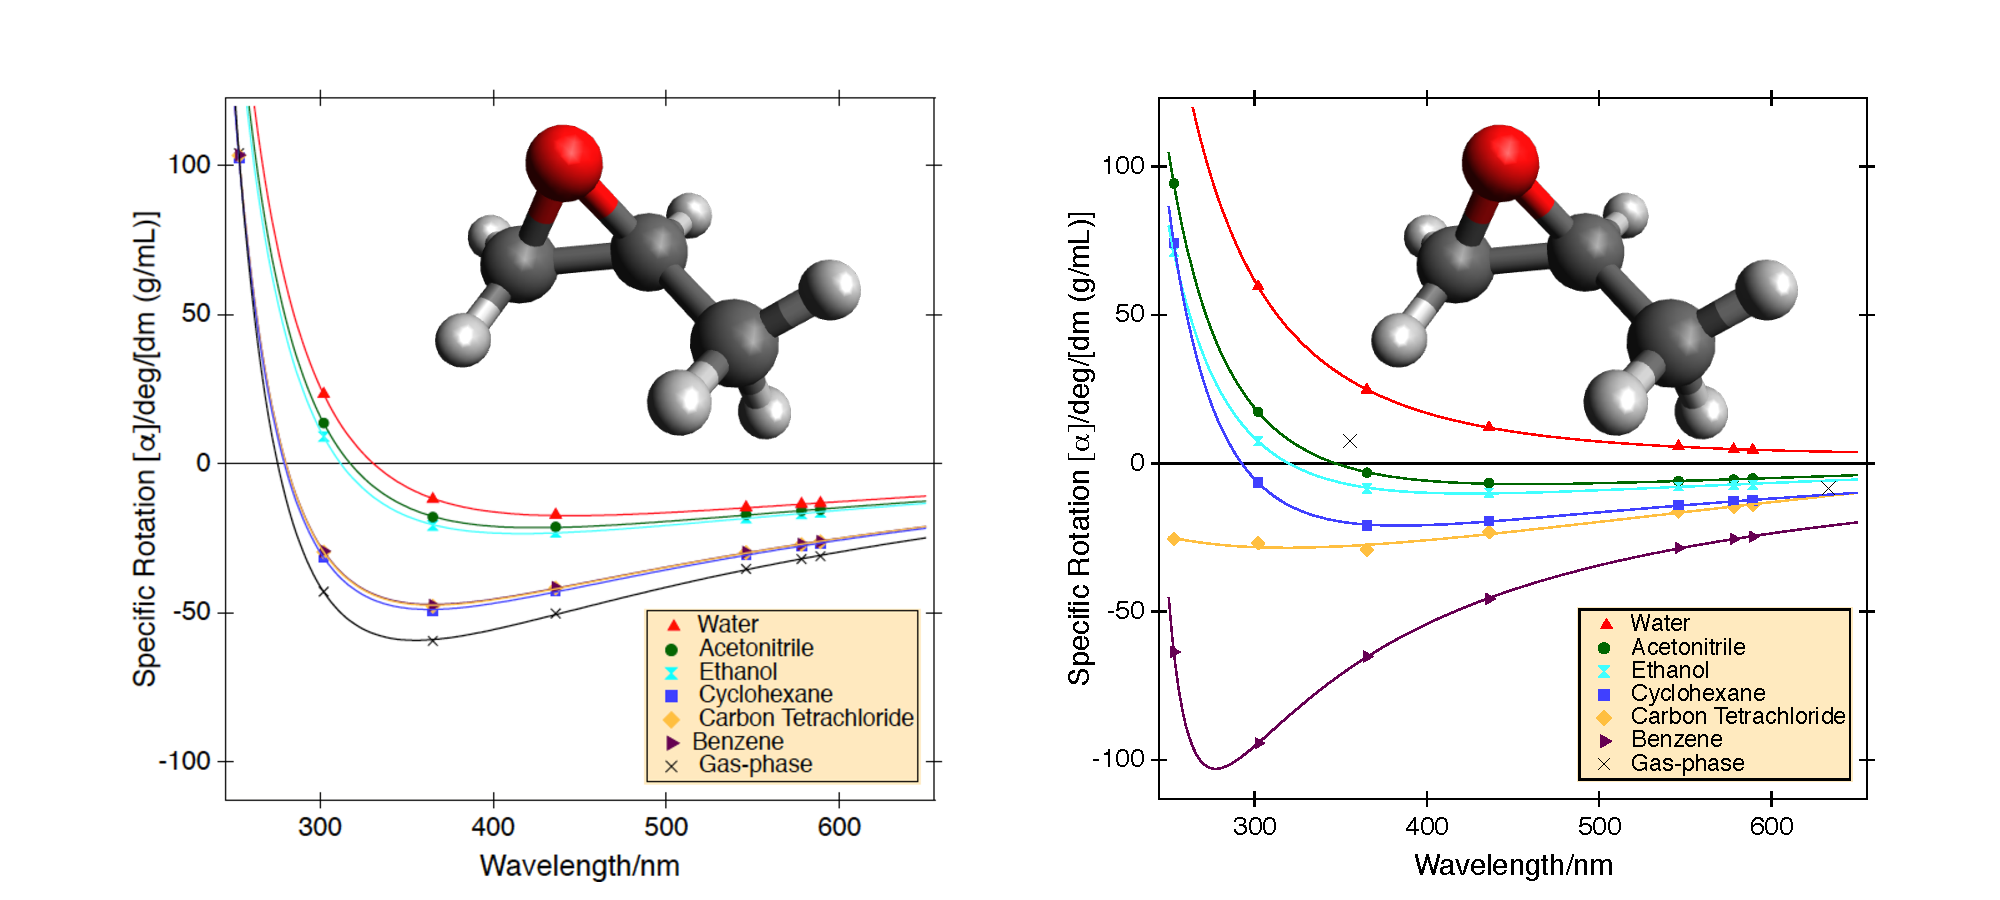
\includegraphics[height=1.75in]{toc.pdf}
     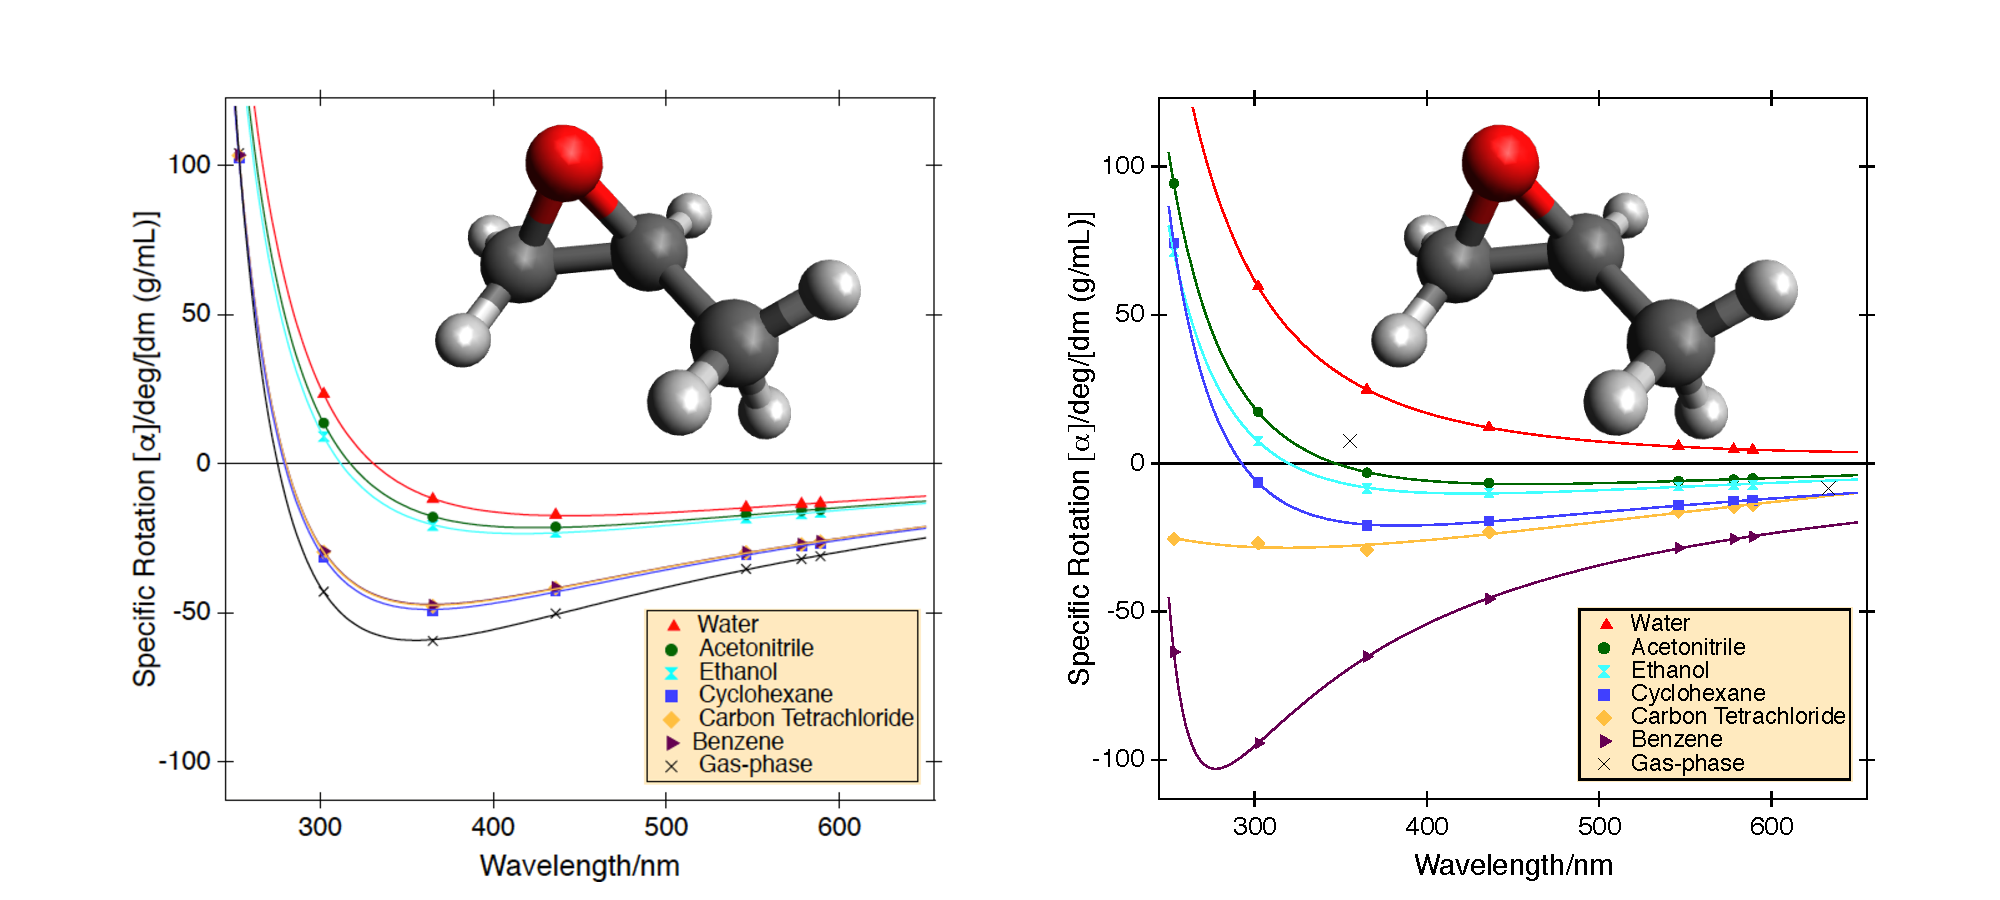
\includegraphics[width=3.25in]{toc.pdf}



 \end{figure}
 \vspace{2cm}
 {\large 
Calculating Optical Rotatory Dispersion Spectra in Solution Using a Smooth
Dielectric Model}
  \vspace{1.5cm} 
  
 {J. Coleman Howard and T. Daniel Crawford}
\end{center}


\end{document}
